\section{Hardness} \label{sec:hardness}
\newcommand{\coord}[3]{v[#1, #2, #3]}
\newcommand{\sepedge}[1]{e^{sep}[#1]}
\newcommand{\varedge}[1]{e^{var}[#1]}
\newcommand{\litedge}[1]{e^{cla}[#1]}

In this section, we establish hardness and inapproximability results for the precedence-constrained covering and decision tree problems introduced in previous sections. Throughout all reductions involving fractional set cover (F-PCSC), we assume that $f = 1$, meaning that each set can be selected at most once.

\subsection{Binary search with precedence constrains}

We begin by showing that the decision tree problem is NP-hard even for the very special of binary searching with precedence. In this problem we are given a linearly ordered set of hypotheses $h_1 \prec h_2 \prec \ldots \prec h_n$ and tests that correspond to binary queries of the form ``Is the unknown hypothesis $h_i$ less than or equal to $h_k$?''. Additionally, a precedence constraints on queries are given which enforce certain queries to be performed before others.

Interestingly, this problem is connected to a seemingly unrelated problem of parallel evaluation of arithmetic expressions. In this problem we are given an arithmetic expression consisting of $n$ variables combined using arbitrary binary operations. Additionally, due to the order of operations of the usage of brackets, a precedence constraints on procesing the operations is given. The goals is to evaluate this expression using arbitrary number of parallel processors however it is required that any operand can undergo only one operation at a time and the precedence constraints are satisfied. The goal is to minimize the total time required to evaluate the expression. It is widely known that without the precedence constraints this problem is equivalent to binary searching on a linearly ordered set of hypotheses. This connection is still valid even when precedence constraints are present, however the precedence constraints on the operations must be reversed. In what follows we show that the problem of binary searching with precedence is NP-hard thereby implying that parallel evaluation of arithmetic expressions with precedence constraints is NP-hard as well.
\begin{theorem}\label{thm:PCWCDT-NP-hard}
    Worst-Case Binary Search With Precedence Constraints is NP-hard.
\end{theorem}
\begin{proof}
	\TP{Bajzel}
	Consider an instance of \ProblemThreeSat given as: a set of variables $V$, and a set of clauses $C$.
	Each clause consist of exactly $3$ literals.
	Moreover, the variant where any $v \in V$ appears at most $5$ times as $v$ or $\overline{v}$ in the clauses is still \NPcomplete \cite{GareyAndJohnson}. 
	Obviously, in this variant $|C| = \cO(|V|)$.
	The idea is to:
	\begin{itemize}
		\item Divide the line into $2$ modules: variables and clauses. 
		Moreover, divide the modules into small segments, so each corresponds to a single variable, clause, respectively.
		Use precedence constraints to force this separation.
		\item All the variable vertices can be queried at the same time.
		Hence, either the variable or it's negation is quarried in a given turn.
		And the negation (or the variable) can be queried in the next.
		\item Make every literal dependent on the corresponding variable.
		\item Now, if at least one variable vertex was queried in the time $t$, then at least one literal vertex can be queried in $t+1$.
		\item If at least one literal vertex was queried then a clause gadget can be quarried in "short" time, because some "middle" vertex of the component was quarried. 
	\end{itemize}
	
	\begin{figure}[htbp]
		\centering
		\begin{tikzpicture}[scale=1.2]
    % Define node styles
    \tikzstyle{vertex}=[circle, fill=blue!40, draw=black, thick, minimum size=6mm]
    \tikzstyle{edge_label}=[font=\small, midway, above]
    \tikzstyle{vertex_label}=[font=\small]
    
    % Title
    \node[font=\large\bfseries, blue!80] at (5, 1) {Clause gadget for $c_i = \{v_i^1, v_i^2, v_i^3\}$};
    
    % Clause gadget for c_i = {v_i^1, v_i^2, v_i^3}
    \node[vertex, label=below:{$v[C,i,1]$}] (c1) at (0, 0) {};
    \node[vertex, label=below:{$v[C,i,v_i^1]$}] (cv1) at (2, 0) {};
    \node[vertex, label=below:{$v[C,i,v_i^{12}]$}] (cv12) at (4, 0) {};
    \node[vertex, label=below:{$v[C,i,v_i^{23}]$}] (cv23) at (6, 0) {};
    \node[vertex, label=below:{$v[C,i,v_i^3]$}] (cv3) at (8, 0) {};
    \node[vertex, label=below:{$v[C,i,2]$}] (c2) at (10, 0) {};
    
    % Draw edges
    \draw[very thick] (c1) -- node[edge_label] {$e^{cla}[i,0]$} (cv1);
    \draw[very thick] (cv1) -- node[edge_label] {$e^{cla}[i,v_i^1]$} (cv12);
    \draw[very thick] (cv12) -- node[edge_label] {$e^{cla}[i,v_i^2]$} (cv23);
    \draw[very thick] (cv23) -- node[edge_label] {$e^{cla}[i,v_i^3]$} (cv3);
    \draw[very thick] (cv3) -- node[edge_label] {$e^{cla}[i,0']$} (c2);
    
    % Precedence annotations
    \node[above=0.5cm of cv1, align=center, font=\footnotesize] (prec1) {depends on\\$e^{var}[v_i^{1,+}]$ or $e^{var}[v_i^{1,-}]$};
    \draw[->, dashed, red, thick] (prec1) -- (cv1);
    
    \node[above=0.5cm of cv23, align=center, font=\footnotesize] (prec3) {depends on\\$e^{var}[v_i^{3,+}]$ or $e^{var}[v_i^{3,-}]$};
    \draw[->, dashed, red, thick] (prec3) -- (cv23);
    
    \node[above=0.3cm of c1, align=center, font=\footnotesize, text=gray] {depends on all\\variable edges};
    \node[above=0.3cm of c2, align=center, font=\footnotesize, text=gray] {depends on all\\variable edges};
    
\end{tikzpicture}

		\caption{Clause gadget for $c_i = \{v_i^1, v_i^2, v_i^3\}$.}
		\label{fig:clause_gadget}
	\end{figure}
	
	\begin{figure}[htbp]
		\centering
		\begin{tikzpicture}[scale=1.2]
    % Define node styles
    \tikzstyle{vertex}=[circle, fill=green!40, draw=black, thick, minimum size=6mm]
    \tikzstyle{edge_label}=[font=\small, midway, above]
    
    % Title
    \node[font=\large\bfseries, green!80] at (3, 1) {Variable gadget for $v_i$};
    
    % Variable gadget for v_i
    \node[vertex, label=below:{$v[v,i,1]$}] (v1) at (0, 0) {};
    \node[vertex, label=below:{$v[v,i,2]$}] (v2) at (3, 0) {};
    \node[vertex, label=below:{$v[v,i,3]$}] (v3) at (6, 0) {};
    
    % Draw edges
    \draw[very thick, green!70!black] (v1) -- node[edge_label, green!70!black] {$e^{var}[v_i^-]$} (v2);
    \draw[very thick, green!70!black] (v2) -- node[edge_label, green!70!black] {$e^{var}[v_i^+]$} (v3);
    
    % Explanation
    \node[above=0.5cm of v2, align=center, font=\footnotesize] {
        Query $e^{var}[v_i^-]$ if $v_i = \text{False}$\\
        Query $e^{var}[v_i^+]$ if $v_i = \text{True}$
    };
    
\end{tikzpicture}

		\caption{Variable gadget for $v_i$.}
		\label{fig:variable_gadget}
	\end{figure}
	
	\begin{figure}[htbp]
		\centering
		%\begin{tikzpicture}[scale=1.0]
    % Define node styles
    \tikzstyle{clauseblob}=[ellipse, fill=blue!30, draw=blue!80, very thick, minimum width=2.5cm, minimum height=1.5cm, font=\small, drop shadow]
    \tikzstyle{varblob}=[ellipse, fill=green!30, draw=green!80, very thick, minimum width=2.5cm, minimum height=1.5cm, font=\small, drop shadow]
    \tikzstyle{sepedge}=[very thick, red]
    
    % Module label
    \node[font=\large\bfseries, blue!80] at (4.25, 1) {Clause module};
    
    % Clause module
    \node[clauseblob] (c1) at (0, 0) {$c_1$\\6 vertices};
    \node[clauseblob] (c2) at (3.5, 0) {$c_2$\\6 vertices};
    \node at (6, 0) {$\cdots$};
    \node[clauseblob] (cC) at (8.5, 0) {$c_{|C|}$\\6 vertices};
    
    % Separator edges between clauses
    \draw[sepedge] (c1) -- node[midway, above, font=\scriptsize, red] {$e^{sep}[1]$} (c2);
    \draw[sepedge] (c2) -- (5, 0);
    \draw[sepedge] (7, 0) -- (cC);
    
    % Connection to variable module
    \draw[sepedge, ->, rounded corners=5mm] (cC.east) -- ++(1, 0) -- ++(0, -2.5) -- ++(-9.5, 0) 
        node[pos=0.5, right, font=\small, text=red] {path\\continues};
    
    % Module label
    \node[font=\large\bfseries, green!80] at (4.25, -4.5) {Variable module};
    
    % Variable module
    \node[varblob] (v1) at (0, -3.5) {$v_1$\\3 vertices};
    \node[varblob] (v2) at (3.5, -3.5) {$v_2$\\3 vertices};
    \node at (6, -3.5) {$\cdots$};
    \node[varblob] (vV) at (8.5, -3.5) {$v_{|V|}$\\3 vertices};
    
    % Separator edges between variables
    \draw[sepedge] (v1) -- node[midway, above, font=\scriptsize, red] {$e^{sep}[|C|+1]$} (v2);
    \draw[sepedge] (v2) -- (5, -3.5);
    \draw[sepedge] (7, -3.5) -- (vV);
    
    % Legend below (centered)
    \node[clauseblob, minimum width=1.2cm, minimum height=0.8cm, font=\footnotesize] at (1, -6) {};
    \node[font=\small] at (3.5, -6) {Clause gadget (6-vertex path)};
    
    \node[varblob, minimum width=1.2cm, minimum height=0.8cm, font=\footnotesize] at (1, -7) {};
    \node[font=\small] at (3.5, -7) {Variable gadget (3-vertex path)};
    
    \draw[sepedge, line width=3pt] (0.5, -8) -- (1.5, -8);
    \node[font=\small] at (3.5, -8) {Separator edge $e^{sep}[i]$};
    
\end{tikzpicture}

		\caption{Overall path structure in the reduction. Clause gadgets are connected by separator edges into a clause module, followed by variable gadgets connected into a variable module. The entire structure forms a single path.}
		\label{fig:reduction_path}
	\end{figure}
	
	\begin{figure}[htbp]
		\centering
		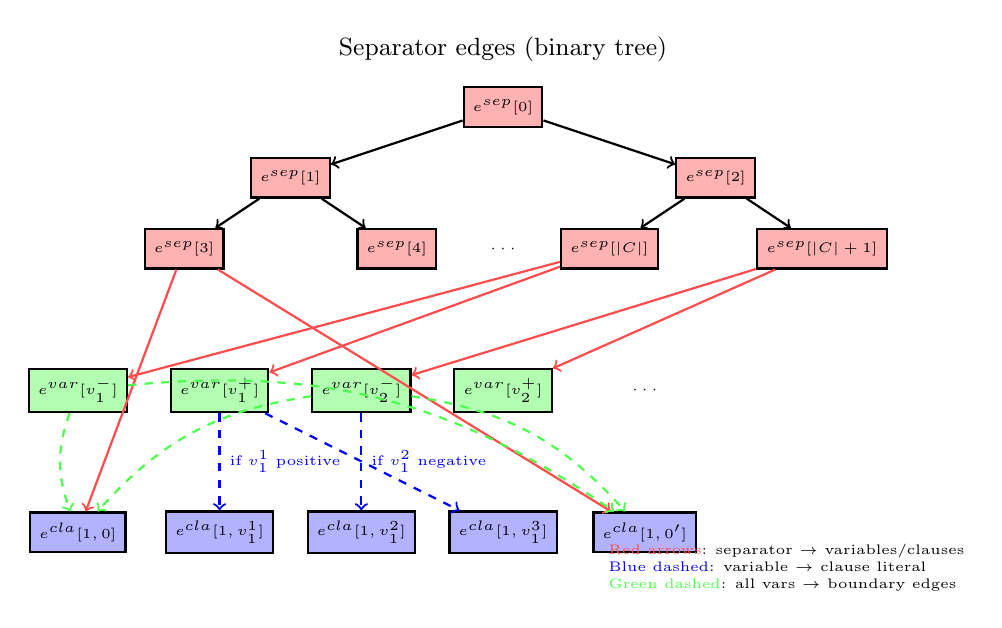
\begin{tikzpicture}[scale=0.9]
    % Define node styles
    \tikzstyle{sepnode}=[rectangle, fill=red!30, draw=black, thick, minimum size=5mm, font=\tiny]
    \tikzstyle{varnode}=[rectangle, fill=green!30, draw=black, thick, minimum size=5mm, font=\tiny]
    \tikzstyle{clanode}=[rectangle, fill=blue!30, draw=black, thick, minimum size=5mm, font=\tiny]
    
    % Top level: Separator edges (binary tree structure)
    \node[sepnode] (sep0) at (6, 5) {$e^{sep}[0]$};
    
    \node[sepnode] (sep1) at (3, 4) {$e^{sep}[1]$};
    \node[sepnode] (sep2) at (9, 4) {$e^{sep}[2]$};
    
    \node[sepnode] (sep3) at (1.5, 3) {$e^{sep}[3]$};
    \node[sepnode] (sep4) at (4.5, 3) {$e^{sep}[4]$};
    \node at (6, 3) {\tiny $\cdots$};
    \node[sepnode] (sep5) at (7.5, 3) {$e^{sep}[|C|]$};
    \node[sepnode] (sep6) at (10.5, 3) {$e^{sep}[|C|+1]$};
    
    % Draw separator tree
    \draw[->, thick] (sep0) -- (sep1);
    \draw[->, thick] (sep0) -- (sep2);
    \draw[->, thick] (sep1) -- (sep3);
    \draw[->, thick] (sep1) -- (sep4);
    \draw[->, thick] (sep2) -- (sep5);
    \draw[->, thick] (sep2) -- (sep6);
    
    \node[above, font=\small] at (6, 5.5) {Separator edges (binary tree)};
    
    % Middle level: Variable edges
    \node[varnode] (var1m) at (0, 1) {$e^{var}[v_1^-]$};
    \node[varnode] (var1p) at (2, 1) {$e^{var}[v_1^+]$};
    \node[varnode] (var2m) at (4, 1) {$e^{var}[v_2^-]$};
    \node[varnode] (var2p) at (6, 1) {$e^{var}[v_2^+]$};
    \node at (8, 1) {\tiny $\cdots$};
    
    % Arrows from separators to variables
    \draw[->, thick, red!70] (sep5) -- (var1m);
    \draw[->, thick, red!70] (sep5) -- (var1p);
    \draw[->, thick, red!70] (sep6) -- (var2m);
    \draw[->, thick, red!70] (sep6) -- (var2p);
    
    % Bottom level: Clause edges
    \node[clanode] (cla10) at (0, -1) {$e^{cla}[1,0]$};
    \node[clanode] (cla1v1) at (2, -1) {$e^{cla}[1,v_1^1]$};
    \node[clanode] (cla1v2) at (4, -1) {$e^{cla}[1,v_1^2]$};
    \node[clanode] (cla1v3) at (6, -1) {$e^{cla}[1,v_1^3]$};
    \node[clanode] (cla10p) at (8, -1) {$e^{cla}[1,0']$};
    
    % Arrows from separators to clause boundary edges
    \draw[->, thick, red!70] (sep3) -- (cla10);
    \draw[->, thick, red!70] (sep3) -- (cla10p);
    
    % Arrows from variables to clause literal edges (precedence constraints)
    \draw[->, thick, blue, dashed] (var1p) -- node[right, font=\tiny] {if $v_1^1$ positive} (cla1v1);
    \draw[->, thick, blue, dashed] (var2m) -- node[right, font=\tiny] {if $v_1^2$ negative} (cla1v2);
    \draw[->, thick, blue, dashed] (var1p) -- (cla1v3);
    
    % Arrows from all variables to boundary edges
    \draw[->, thick, green!70, dashed] (var1m) to[bend right=20] (cla10);
    \draw[->, thick, green!70, dashed] (var2m) to[bend right=20] (cla10);
    \draw[->, thick, green!70, dashed] (var1m) to[bend left=20] (cla10p);
    \draw[->, thick, green!70, dashed] (var2m) to[bend left=20] (cla10p);
    
    % Legend
    \node[align=left, font=\tiny] at (10, -1.5) {
        \textcolor{red!70}{Red arrows}: separator $\to$ variables/clauses\\
        \textcolor{blue}{Blue dashed}: variable $\to$ clause literal\\
        \textcolor{green!70}{Green dashed}: all vars $\to$ boundary edges
    };
    
\end{tikzpicture}

		\caption{Precedence constraints DAG. Separator edges form a binary tree (top), which precede all variable edges (middle) and clause edges (bottom). Blue dashed arrows show precedence from variable edges to clause literal edges, green dashed arrows show that all variable edges precede clause boundary edges.}
		\label{fig:reduction_precedence}
	\end{figure}
	
	More formally, the mapping of an instance of \ProblemThreeSat given as a set of clauses, denoted by $C$, and variables, denoted by $V$, is as follows.
	To construct all other edges e graph:
	\begin{enumerate}
		\item Let $d > 0$ be smallest value such a value that $\log_2(|C| + |V| - 2 + d) \in Z$.
		Add $d$ dummy variables -- i.e. variables unrelated to any clause.
		From now, we assume that $|V| + |C| - 1 = 2^k-1$, for some $k > 0$.
		\item For every $c_i = \{v_i^1, v_i^2, v_i^3\}$, construct a gadget given as a path graph on vertices
		\[
			\coord{C}{i}{1}, \coord{C}{i}{v_i^1}, \coord{C}{i}{v_i^{12}}, \coord{C}{i}{v_i^{23}}, \coord{C}{i}{v_i^3}, \coord{C}{i}{2}.
		\]
		Denote the edges between the consecutive pairs of vertices as: $\litedge{i, 0}$, $\litedge{i, v_i^1}$, $\litedge{i, v_i^2}$, $\litedge{i, v_i^3}$, $\litedge{i, 0'}$.
		\item For a variable $v_i$, construct a gadget compose of $3$ vertices as a path
		\[
			\coord{v}{i}{1}, \coord{v}{i}{2}, \coord{v}{i}{3}
		\]
		Denote the edge $(\coord{v}{i}{1}, \coord{v}{i}{2})$ as $\varedge{v_i^-}$.
		Denote the edge $(\coord{V}{v}{2}, \coord{v}{i}{3})$ as $\varedge{v_i^+}$.
		\item Compose the graph in the following way.
		Connect each clause gadget one by one, let the vertex $\coord{C}{i}{4}$ is connected to $\coord{C}{i+1}{1}$ by and edge denoted as $\sepedge{i}$.
		Let us denote such an edge from this set as "separator edge".
		Connect $\coord{ M_{SAT}^*(I_S)C}{|C|}{4}$ to $\coord{V}{i}{1}$ by $\sepedge{|C|}$, $C$-th separator edge.
		Continue with variable gadgets in the same way; hence the total number of separator edges is $|C| + |V| - 1$.
	\end{enumerate}
	To define the order on the edges:
	\begin{enumerate}
		\item There are exactly $1+2+\ldots+2^{k}$ separator edges, for some $k > 0$.
		Hence easily one can make an order corresponding to binary tree, to force the queries.
		\item Force all other edges to be preceded by the separator edges.
		\item For every clause $C_i$ and every $v \in \{v_i^1,v_i^2,v_i^3\}$ make $\litedge{i, v}$ dependent on $\varedge{v^+}$ if $v$ is positive literal; make it dependent on $\varedge{v^-}$ otherwise.
		\item For every clause $C_i$, make $\litedge{i, 0}$ and $\litedge{i, 0'}$ dependent on all variable edges.
	\end{enumerate}
	Now, to prove that the problem is \NPhard we prove the decision version of the problem is \NPcomplete, 
	i.e. the problem to determine if for a given input $(P, O, t)$ there exists a strategy of maximum search time less than or equal to $t$.
	
	To prove that the problem is in \NP we observe that given search tree certifies maximum search time.
	
	Now, assume that the instance of $(C, V)$ \ProblemThreeSat is of 'YES' type.
	Hence let $f: V \leftarrow \{T, F\}$ be a valuation which satisfies all the clauses.
	Then, we build the strategy:
	\begin{itemize}
		\item Query the separator edges in time up to $k$.
		\item For every variable-vertex $v$, if variable was assigned $T$, query $\varedge{v^+}$ it in time $k+1$; otherwise query $\varedge{v^-}$.
		      Hence, they are queried in times $k+1$ and $k+2$, respectively. 
		\item Now all the clause gadgets have at least one precondition met in time $k+1$.
		      Due to this we can query at least one of $\litedge{i, v_i^1}$, $\litedge{i, v_i^2}$, $\litedge{i, v_i^3}$ in time $k+2$.
		      Due to the fact that for each clause there are up to $4$ candidate vertices, and each edge can be queried freely in time $k+3$ or later we can complete the queries in time up to $k+4$.
	\end{itemize}
	Due to this for the constructed graph there exists a strategy of time $k+4$.
	
	Assume now that the answer for the constructed instance, i.e. path graph, order, and time $k+4$ the answer is 'YES'.
	We perform the following observations.
	\begin{itemize}
		\item For a given clause-gadget corresponding, due to the fact that there are $5$ edges, we need at least $3$ time units to query it. 
		\item The earliest possible time to finish querying the separator edges is $k$.
		\item Due to this we have to perform at least one query in time $k+2$ for every clause-gadget $c_i$.
		Due to the fact that $\litedge{i, 0}$ and $\litedge{i, 0'}$ cannot be queried before $k+3$, it has to be the case that one of $\litedge{i, v_i^1}$, $\litedge{i, v_i^2}$, $\litedge{i, v_i^3}$ was queried.
		Hence, at for at least one of the edges preconditions were met (edge was queried) in time $k+1$.
		The variable-edges queried in $k+1$ to a valuation of the variables matching all the clauses.
	\end{itemize}
	
\end{proof}


\begin{theorem}
    Average-Case Binary Search With Precedence Constraints is \NPhard.
\end{theorem}
\begin{proof}
	The reduction is the same as in the worst-case variant; except that we have to consider the total query time.
	Again assume that the instance of \ProblemThreeSat is of 'YES' type.
	As previously, let $\log_2(|C| + |V|) = k$, hence $k \le 3 + \log_2m$.
	Hence:
	\begin{itemize}
	\item In any reasonable solution the separator-edges will have total quarry time $1 + 2*2 + 4*3 + 8*4 + \ldots 2^k*k$, denoted by $T_{sep}$.
	\item 	Now, the $|V|$ variable-edges correspond to total quarry time $|V| (2k+3)$, denoted by $T_{var}$.
	\item After this, consider the total quarry time of clause edges. 
	For a satisfied clause, there can be one quarry in time $k+2$ and other quarries $4$ can be done in time $k+3, k+3, k+4, k+4$. 
	Hence this gives total quarry time $|C|(5k + 16)$, denoted by $T_{clauses}$.  
	\end{itemize} 
	Together it gives the total quarry time $T_{sep} + T_{var} + T_{clauses}$ in a search tree corresponding to a valuation of variables satisfying all the clauses.
	The reverse direction, that a search tree of total quarry time $T_{sep} + T_{var} + T_{clauses}$ corresponds to a valuation satisfying all the clauses, is left to the reader.
	
\end{proof}
	
\begin{theorem}
		Worst-Case Tree Search With Precedence Constraints is cannot be approximated with ration better than $\frac{}{}$ unless $\Pclass = \NP$.
\end{theorem}
\begin{proof}
	The reduction is very similar to the previous ones, albeit we the path graph with a tree graph.  
\end{proof}

\begin{theorem}
	Average-Case Tree Search With Precedence Constraints is cannot be approximated with ration better than $\frac{}{}$ unless $\Pclass = \NP$.
\end{theorem}
\begin{proof}
	However, to prove hardness we make an $L$-reduction from \ProblemMaxThreeSat.
	For the formal definition of the reduction we recommend \cite{Ausiello}.
	Namely, the problem where we would like to maximize the number of fulfilled clauses.
	To prove this we have to provide functions:
	\begin{itemize}
		\item $f$ -- mapping from the instances of \ProblemMaxThreeSat to Binary Search.
		\item $g$ -- mapping from the solutions of Binary Search to the solutions of \ProblemMaxThreeSat. 
	\end{itemize}
	And we need to prove the 2 crucial properties (other properties mentioned in the referenced definition are straightforward).
	For the first one, 
	let $I_S$ be any instance of \ProblemMaxThreeSat,
	let $f(I_S)$ -- the constructed instance of \ProblemAverageCaseBinarySearchPrecedanceConstraints,
	and let, $M_{SEARCH}$ and $M_{SAT}$ be the optimality measures for the respective problems (for the respective problems), also let $M_{SEARCH}^*$ and $M_{SEARCH}^*$ be the values of the optimal solutions for the instance.
	The property to prove is
	\[
	M_{SEARCH}^*(f(I_S)) \le \beta M_{SAT}^*(I_S)
	\]
	for some fixed $\beta > 0$.
	To prove this, we observe: 
	\begin{itemize}
		\item On one hand for any $I_S$ composed of $m$ clauses, we can observe at once that $M_{SAT}^*(I_S) \ge m/2$.
		\item On the other hand for such an instance, we can drop all variables which do not appear in any clause. 
		Due to this the number of variables is bounded by $3m$.
		Hence, for the instance, due to the dummy variables, $|C| + |V| \le 8m$.
		As previously, let $\log_2(|C| + |V|) = k$, hence $k \le 3 + \log_2m$.
		Hence, in an optimal solution the separator-edges will have total quarry time $1 + 2*2 + 4*3 + 8*4 + \ldots 2^k*k = C_{sep}$.
		\item Now, the $|V|$ variable-edges correspond to total quarry time $|V| (2k+3) = C_{var}$.
		\item After this, consider the total quarry time of clause edges. 
		For a satisfied clause, there can be one quarry in time $k+2$ and other quarries $4$ can be done in time $k+3, k+3, k+4, k+4$. 
		Hence this gives total quarry time $|C|(5k + 16)$ = $C_{clauses}$. 
	\end{itemize}
\end{proof}


\subsection{Outforest precendce constrains}
\begin{theorem}\label{thm:PCSC-to-PCWCDT-hardness}
    If there is no $\alpha$-approximation for \ProblemPCSC, then there is no $\cO\br{\alpha}$-approximation for \ProblemPCWCDT.
\end{theorem}
\begin{proof}
    Let $(U, \mathcal{S}, P)$ be an instance of \ProblemPCSC\ where $U$ is the universe of elements, $\mathcal{S}$ is the family of sets and $P$ are the precedence constraints on $\mathcal{S}$. We construct an instance of \ProblemPCWCDT\ as follows. For each element $u \in U$, we create two representative hypotheses $h_u^0$ and $h_u^1$. For each set $S \in \mathcal{S}$, we create a test $t_S$ such that $t_S(h_u^i) = h_u^i$ if $u \in S$ and $t_S(h_u^i) = 0$ otherwise. The precedence constraints on tests are the same as the precedence constraints on sets, i.e., if $S_1$ must be selected before $S_2$ in \ProblemPCSC, then $t_{S_1}$ must be selected before $t_{S_2}$ in \ProblemPCWCDT. Notice, that any valid decision tree for the constructed instance of \ProblemPCWCDT\ is a path of tests (ignoring leafs) since performing any test $t_S$ either returns a response containing one of the hypotheses $h_u^i$, thus ending a process or returns $0$, which is a singular possible response leading to the next test. Note that even when the candidate set contains only representatives of one element $u$, we still need to perform a test to distinguish between $h_u^0$ and $h_u^1$, which could not be a case if there was only one hypothesis per element.
    Therefore, any valid decision tree for the constructed instance of \ProblemPCWCDT\ corresponds to a valid selection of sets in \ProblemPCSC\ and vice versa. Moreover, the cost of the decision tree is equal to the number of selected sets. Thus, since the size of the reduction is linear any $\alpha$-approximation for \ProblemPCWCDT\ would yield an $\cO\br{\alpha}$-approximation for \ProblemPCSC.
\end{proof}
\begin{theorem}\label{thm:PCMSSC-to-PCACDT-hardness}
    If there is no $\alpha$-approximation for $\ProblemPCMSSC$, then there is no $\cO\br{\alpha}$-approximation for $\ProblemPCACDT$.
\end{theorem}
\begin{proof}
    We use the same reduction as in the previous theorem. Note that since we doubled the number of hypotheses in the construction, the cost of any decision tree in the constructed instance of \ProblemPCACDT\ is twice the number of selected sets in \ProblemPCMSSC. However, this does not affect the structure of the reduction and thus any $\alpha$-approximation for \ProblemPCACDT\ would yield an $\cO\br{\alpha}$-approximation for \ProblemPCMSSC.
\end{proof}
\begin{theorem}\label{thm:PCSC-to-PCACDT-hardness}
    If there is no $\alpha$-approximation for $\ProblemPCSC$, then there is no $\cO\br{\alpha}$-approximation for $\ProblemPCACDT$.
\end{theorem}
\begin{proof}
	Let $(U, \mathcal{S}, P)$ be an instance of \ProblemPCSC\ where $U$ is the universe of elements, $\mathcal{S}$ is the family of sets and $P$ are the precedence constraints on $\mathcal{S}$. We construct an instance of $\ProblemPCACDT$ as follows. For each element $u \in U$, we create a representative hypothesis $h_u$ with $p\br{h_u}=0$. We also create a dummy hypothesis $h$ such that $p\br{h}=1$. For each set $S \in \mathcal{S}$, we create a test $t_S$ such that $t_S(h_u) = h_u$ if $u \in S$ and $t_S(h_u) = 0$ otherwise ($t_S(h)=0$). The precedence constraints on tests are the same as the precedence constraints on sets, i.e., if $S_1$ must be selected before $S_2$ in \ProblemPCSC, then $t_{S_1}$ must be selected before $t_{S_2}$ in \ProblemPCWCDT. Notice, that any valid decision tree for the constructed instance of \ProblemPCWCDT\ is a path of tests (ignoring leafs) since performing any test $t_S$ either returns a response containing one of the hypotheses $h_u$, thus ending a process or returns $0$, which is a singular possible response leading to the next test. Since the dummy hypothesis $h$ has probability $1$, the cost of any decision tree is equal to the number of tests performed in the path. In order to distinguish all hypotheses $h_u$ from the dummy hypothesis $h$, we need to perform tests that cover all elements in $U$.
    Therefore, any valid decision tree for the constructed instance of \ProblemPCWCDT\ corresponds to a valid selection of sets in \ProblemPCSC\ and vice versa. Thus, since the size of the reduction is linear any $\alpha$-approximation for \ProblemPCWCDT\ would yield an $\cO\br{\alpha}$-approximation for \ProblemPCSC.
\end{proof}
\subsection{Outforest precedence constraints}
\begin{theorem}\label{thm:PCSC-outforest-hardness}
    $\ProblemPCSC$ with outforest precedence constraints is NP-hard to approximate within a factor of $\cO\br{\log^{2-\epsilon} n}$ for any $\epsilon > 0$ unless $\text{NP}\subseteq \text{ZTIME}\br{n^{\text{polylog}(n)}}$.
\end{theorem}
\begin{proof}
    To show this we prove that Group Steiner Tree on tree metrics is reducible to Set Cover with outforest precedence constraints. Since GST on trees cannot be approximated within a factor of $\cO\br{\log^2 n}$ unless $\text{NP}\subseteq \text{ZTIME}\br{n^{\text{polylog}(n)}}$ \cite{PolylogarithmicInapproximability}. Note that in the latter reduction all of the weights are of form $2^{-h}$ with exponent ranging from $0$ to $h=\cO\br{\log^{1-\epsilon} n}$. Therefore, we can scale all weights by $2^h=\text{poly}\br{n}$ to obtain integer weights without affecting the approximation ratio. Let $T, w, \mathcal{G}$ be an instance of GST where $T$ is a tree metric with root $r$, $w$ are the weights on the edges of $T$ and $\mathcal{G}=\br{G_1, \ldots, G_k}$ are the groups. We construct an instance of \ProblemPCSC\ with outforest precedence constraints as follows. Since to include a node in the Steiner Tree we need to include its parent edge of cost $w_e$, for each vertex $v\neq r$ we create its $w_e$ representatives $S_v^1 \preceq \ldots \preceq S_v^{w_e}$ so that taking $S^{w_e}$ to the cover requires taking all of the previous representatives. Additionally, for any directed edge $uv\in E$ such that $u \neq r$ and $e$ is a parent edge of $u$, we set $S^{w_e}_u \preceq S^1_v$ to enforce the condition that to including a node in a Steiner Tree requires including its parent node with its parent edge. For each group $G_i$ we create a universe element $u_i$. If $v \in G_i$ and $e$ is the parent edge of $v$, we set $S_{w_e}$ to cover $u_i$. It is easy to see that in order to cover any universe element by a vertex $v$ one needs to include all representatives of ancestors of $v$ excluding $r$. Therefore, any valid selection of sets in the constructed instance of \ProblemPCSC\ corresponds to a valid Steiner Tree in the instance of GST and vice versa. Moreover, the cost of the selected sets is equal to the cost of the Steiner Tree. Thus, \ProblemPCSC\ with outforest precedence constraints cannot be approximated within a factor of $\cO\br{\log^{2-\epsilon} n}$ for any $\epsilon > 0$ unless $\text{NP}\subseteq \text{ZTIME}\br{n^{\text{polylog}(n)}}$.
\end{proof}
As an immediate corollaries of Theorem \ref{thm:PCSC-to-PCWCDT-hardness} and \ref{thm:PCSC-to-PCWCDT-hardness} we obtain the following results:
\begin{corollary}\label{thm:PCWCDT-outforest-hardness}
    $\ProblemPCWCDT$ with outforest precedence constraints is NP-hard to approximate within a factor of $\cO\br{\log^{2-\epsilon} n}$ for any $\epsilon > 0$ unless $\text{NP}\subseteq \text{ZTIME}\br{n^{\text{polylog}(n)}}$.
\end{corollary}

\begin{corollary}\label{thm:PCACDT-outforest-hardness}
    $\ProblemPCACDT$ with outforest precedence constraints is NP-hard to approximate within a factor of $\cO\br{\log^{2-\epsilon} n}$ for any $\epsilon > 0$ unless $\text{NP}\subseteq \text{ZTIME}\br{n^{\text{polylog}(n)}}$.
\end{corollary}

\subsection{General precedence constraints}
In this section we show strong inapproximability results for \ProblemPCWCDT\ and \ProblemPCACDT\ with general precedence constraints by reducing from the Planted Dense Subgraph Conjecture which is a widely believed statement about hardness of detecting a dense component within an Erdős-Renyi graph \cite{OnApproxTargetSetSelection,PCMSSC}.
\begin{conjecture}[Planted Dense Subgraph (PDS) Conjecture] \label{problem:PDS}
For any constants $\beta < \alpha$ and any $k\geq \sqrt{N}$, there is no polynomial time algorithm that can distinguish between the following two distributions of graphs with any advantage $\epsilon > 0$: (1) With probability 1/2, an Erdős-Renyi graph $G(N, N^{\alpha - 1})$, (2) With probability 1/2, an Erdős-Renyi graph $G(N, N^{\alpha - 1})$ with a planted subgraph of size $k$ and edge density $k^{\beta - 1}$.
\end{conjecture}
\DD{DD: tutaj wkleiłem conjecture i zakomentowałem jej parafrezę (możemy podmienić, ale nie ma sensu mieć obu).}
% The Planted Dense Subgraph Conjecture states that for any constants $ \beta < \alpha $ and any $k\geq \sqrt{N}$, there is no polynomial time algorithm that can distinguish between the following two distributions of graphs with any advantage $\epsilon > 0$:
% \begin{itemize}
%     \item With probability 1/2, $G_1$: an Erdős-Renyi graph $G(N, N^{\alpha - 1})$,
%     \item With probability 1/2, $G_2$: an Erdős-Renyi graph $G(N, N^{\alpha - 1})$ with a planted subgraph of size $k$ and edge density $k^{\beta - 1}$.
% \end{itemize}
Using this conjecture one can show the following inapproximability results for \ProblemPCMSSC\ \cite{PCMSSC}:
\begin{theorem}\label{thm:PCMSSC-PDS-hardness}
    For any $\epsilon>0$ \ProblemPCMSSC\ cannot be approximated within a factor of $\cO\br{m^{1/6-\epsilon}}$ nor $\cO\br{n^{1/12-\epsilon}}$ condition to Planted Dense Subgraph Conjecture.
\end{theorem}
Using the reduction from \ProblemPCMSSC\ to \ProblemPCACDT\ and \ProblemPCWCDT\ from the previous section we immediately obtain the following results:
\begin{corollary}\label{thm:PCACDT-PDS-hardness}
    For any $\epsilon>0$ $\ProblemPCACDT$ cannot be approximated within a factor of $\cO\br{m^{1/6-\epsilon}}$ nor $\cO\br{n^{1/12-\epsilon}}$ condition to Planted Dense Subgraph Conjecture. 
\end{corollary}

Below we show that a similar reduction can also be used to obtain the same inapproximability result for \ProblemPCSC. In the reduction we will often make use of the Chernoff Bound which is as follows:
\begin{theorem}[Chernoff Bound]\label{thm:chernoff}
    Let $X_1, X_2, \ldots, X_n$ be independent random variables taking values in $\brc{0,1}$ such that for every $i\in\{1,\ldots,n\}$, $\mathbb{P}[X_i=1]=p$. Let $X=\sum_{i=1}^n X_i$ and $\mu=\mathbb{E}[X]=pn$. Then, for every $\delta\in(0,1)$ it holds that:
    \begin{align*}
        \mathbb{P}[X\leq (1-\delta)\mu] &\leq e^{-\frac{\delta^2\mu}{2}},\\
        \mathbb{P}[X\geq (1+\delta)\mu] &\leq e^{-\frac{\delta^2\mu}{3}}.
    \end{align*}
\end{theorem}

We have the following theorem:
\begin{theorem}\label{thm:PCSC-PDS-hardness}
    For any $\epsilon>0$ PCSC cannot be approximated within a factor of $\cO\br{m^{1/6-\epsilon}}$ nor $\cO\br{n^{1/12-\epsilon}}$ condition to Planted Dense Subgraph Conjecture.
\end{theorem}
\begin{proof}
    \paragraph{Construction of the reduction.} We start by choosing appropriate parameters for our reduction. Let $k=\sqrt{N}$, $\alpha=1/2$ and $\beta=1/2-\gamma$ for some $\gamma > 0$ to be determined later. In our reduction we will embed the structure of the input graph into the precedence constraints, while the universe elements will enforce the covering requirement. 
    
    Given a graph $G=(\{1,\ldots,N\}, \mathcal{E})$ as input to the Planted Dense Subgraph problem, we construct an instance of PCSC as follows. For each vertex $v \in \{1,\ldots,N\}$ of $G$, we create $\lambda$ representative sets $V_{v, i}$ for $i \in \{1,\ldots,\lambda\}$, where $\lambda$ is an appropriately chosen natural number to be specified later. For each edge $uv\in\mathcal{E}$, we create one representative set $E_{uv}$ which must be preceded by all representatives of both $u$ and $v$. That is, for all $i \in \{1,\ldots,\lambda\}$, we have $V_{u, i} \preceq E_{uv}$ and $V_{v, i} \preceq E_{uv}$. 

    Next, we define the universe of elements to be covered. Let $U=\{0,1,\dots, n\}$ for some appropriately chosen natural number $n$ to be determined later. Every vertex representative set contains only the special element $0$, that is, $V_{v, i}=\{0\}$ for all $v \in \{1,\ldots,N\}$ and $i \in \{1,\ldots,\lambda\}$. 
    
    To define the contents of edge representative sets, we use a randomized construction based on a parameter $p\in(0,1)$. For each vertex $v \in \{1,\ldots,N\}$, we define an auxiliary set $U_v \subseteq \{1,\dots, n\}$ by including each element $j \in \{1,\dots, n\}$ in $U_v$ independently with probability $p$. That is, for each $j \in \{1,\dots, n\}$ and each $v \in \{1,\ldots,N\}$, we have $\mathbb{P}[j \in U_v] = p$. The edge representative set $E_{uv}$ is then defined to cover the intersection of the auxiliary sets of its endpoints together with the special element, that is, $E_{uv} = \{0\} \cup (U_u \cap U_v)$. 
    
    From this construction, we can compute the following expected values:
    \begin{itemize}
        \item $\mathbb{E}[\spr{U_v}] = p n$ for each vertex $v$,
        \item $\mathbb{E}[\spr{\{v\colon j\in U_v\}}] = p N$ for each element $j \in \{1,\dots, n\}$,
        \item $\mathbb{E}[\spr{E_{uv}}] = 1 + \mathbb{E}[\spr{U_u \cap U_v}] = 1 + np^2$ for each edge $uv$.
    \end{itemize}

    The intuition behind this construction is as follows: we choose $p$ to be the smallest value such that if a planted component exists, then with high probability it covers all of $U$ using only edge representatives from the planted component (and their required predecessors). On the other hand, if no planted component exists, then we show that any solution must use significantly more sets to cover $U$, thus establishing the desired inapproximability ratio. 
    
    \paragraph{Choice of parameters.}
    Let $\mathcal{P}$ denote the planted component if it exists. Since $\mathcal{P}$ consists of $k = \sqrt{N}$ vertices, for any element $j \in \{1,\dots, n\}$, the expected number of vertices in $\mathcal{P}$ whose auxiliary sets contain $j$ is $\mathbb{E}[\spr{\{v\colon j\in U_v, v \in V(\mathcal{P})\}}] = p\sqrt{N}$. Therefore, the expected number of unordered pairs of vertices in $\mathcal{P}$ where both auxiliary sets contain $j$ is:
    $$
    \mathbb{E}\left[\left|\left\{(v, u)\colon j\in U_v, j\in U_u, v,u \in V(\mathcal{P}), v < u\right\}\right|\right] = \binom{p\sqrt{N}}{2}.
    $$
    
    Since each edge in $\mathcal{P}$ exists independently with probability $k^{\beta - 1} = (\sqrt{N})^{-1/2 - \gamma}=N^{-1/4-\gamma/2}$, the expected number of edge representative sets from $\mathcal{P}$ that cover element $j$ is:
    $$
    \mathbb{E}[\spr{\{E_{uv}\colon j\in E_{uv}, uv \in E(\mathcal{P})\}}] = \binom{p\sqrt{N}}{2} \cdot N^{-1/4-\gamma/2}\geq \frac{p^2N}{4} \cdot N^{-1/4-\gamma/2}=\frac{p^2 N^{3/4-\gamma/2}}{4}.
    $$ 
    For this expected value to be sufficiently large (specifically, to be $\Theta(\log^2 N)$), we choose:
    $
    p=32\cdot N^{-3/8+\gamma/4}\cdot \log N
    $. 
	We have $\mathbb{E}[\spr{\{E_{uv}\colon j\in E_{uv}, uv \in E(\mathcal{P})\}}] \geq 64\log^2 N$, which will allow us to apply concentration bounds effectively.

    \paragraph{Case 1: Planted component exists.} Assume that the input graph contains a planted component $\mathcal{P}$. We show that there exists a solution to PCSC using only sets corresponding to vertices and edges in $\mathcal{P}$ that covers all elements in $U$ with high probability, and that this solution has cost $O(\lambda\sqrt{N}+N^{3/4-\gamma/2})$.
    Consider the solution that selects all vertex representatives $V_{v,i}$ for all $v \in V(\mathcal{P})$ and all $i \in [\lambda]$, together with all edge representatives $E_{uv}$ for all edges $uv \in E(\mathcal{P})$. The special element $0$ is covered by any vertex representative, so we focus on covering elements in $\{1,\dots, n\}$.
    
    Fix an arbitrary element $j \in \{1,\dots, n\}$. We first bound the number of vertices in $\mathcal{P}$ whose auxiliary sets contain $j$. Since $\mathbb{E}[\spr{\{v\colon j\in U_v, v \in V(\mathcal{P})\}}] = p\sqrt{N}$, by Chernoff's bound (Theorem \ref{thm:chernoff}) with $\delta = 1/2$, we have:
    $$
    \mathbb{P}\left[\left|\{v\colon j\in U_v, v \in V(\mathcal{P})\}\right| \leq \frac{p\sqrt{N}}{2}\right] \leq  e^{-p\sqrt{N}/8} = e^{-4\cdot N^{1/8+\gamma/4}\cdot \log N} = N^{-4\cdot N^{1/8+\gamma/4}},
    $$
    which is exponentially small. 
    
    Next, for large enough $x$, we have $\binom{x}{2} \geq x^2/4$. Therefore, the expected number of unordered pairs of vertices in $\mathcal{P}$ where both auxiliary sets contain $j$ is at least $p^2N/4$. Again by Chernoff's bound, we have:
    $$
    \mathbb{P}\left[\left|\{(u,v)\colon j\in U_u, j\in U_v, u,v \in V(\mathcal{P}), u < v\}\right| \leq \frac{p^2N}{16}\right] \leq N^{-4\cdot N^{1/8+\gamma/4}}.
    $$

    Now, each such pair $(u,v)$ corresponds to an edge in $\mathcal{P}$ with probability $N^{-1/4-\gamma/2}$. Since edge existence is independent of the auxiliary set memberships, the expected number of edge representatives in $\mathcal{P}$ that cover $j$ is:
    $$
    \mu := \mathbb{E}[\spr{\{E_{uv}\colon j\in E_{uv}, uv\in E(\mathcal{P})\}}] \geq \frac{p^2N}{16} \cdot N^{-1/4-\gamma/2}=64\log^2 N.
    $$

    Applying Chernoff's bound once more, we obtain:
    $$
    \mathbb{P}[\spr{\{E_{uv}\colon j\in E_{uv}, uv\in E(\mathcal{P})\}} \leq \mu/2] \leq e^{-\mu/8} = e^{-8\log^2 N} = N^{-8\log N}.
    $$

    By the union bound over all $n$ elements in $\{1,\dots, n\}$, the probability that some element is not covered by the edge representatives in $\mathcal{P}$ is at most $n \cdot N^{-8\log N}$. We will choose $n = \Theta(N^{3/4})$ later, which makes this probability negligible for large $N$.
    
    Finally, we bound the number of sets in this solution. The number of vertex representative sets is exactly $\lambda\sqrt{N}$. For the edge representatives, observe that:
    $$
    \mathbb{E}[\spr{E(\mathcal{P})}]=\binom{\sqrt{N}}{2}\cdot N^{-1/4-\gamma/2}\leq \frac{N}{2} \cdot N^{-1/4-\gamma/2} = \frac{N^{3/4-\gamma/2}}{2}.
    $$
    
    By Chernoff's bound with $\delta = 1$, we have:
    $$
    \mathbb{P}[\spr{E(\mathcal{P})} \geq N^{3/4-\gamma/2}] \leq e^{-N^{3/4-\gamma/2}/6},
    $$
    which is extremely small. Therefore, with high probability, the total number of sets in the solution is at most:
    $$
    \lambda\sqrt{N}+N^{3/4-\gamma/2}.
    $$
    
    \paragraph{Case 2: No planted component.} Now assume that the input graph does not contain a planted component, so it is drawn entirely from $G(N, N^{-1/2})$. We show that any solution to PCSC must use significantly more sets to cover all elements in $U$ with high probability.
    
    Consider any solution to PCSC that selects representatives corresponding to some set $X \subseteq \{1,\ldots,N\}$ of vertices with $|X| = x$. Due to the precedence constraints, this solution must include all $\lambda x$ vertex representatives $V_{v,i}$ for $v \in X$ and $i \in \{1,\ldots,\lambda\}$. After selecting these vertex representatives, the solution can then select edge representatives $E_{uv}$ for edges $uv$ where both $u, v \in X$.
    
    We first bound the number of edges among the vertices in $X$. Since the graph is drawn from $G(N, N^{-1/2})$, each potential edge exists independently with probability $N^{-1/2}$. For any fixed set $X$ of size $x$, the expected number of edges with both endpoints in $X$ is:
    $$
    \mu_E := \binom{x}{2}\cdot N^{-1/2} \leq \frac{x^2}{2\sqrt{N}}.
    $$
    
    There are at most $\binom{N}{x} \leq N^x$ possible sets $X$ of size $x$. By Chernoff's bound with $\delta = 1/2$, the probability that a specific set $X$ contains more than $3\mu_E/2$ edges is at most $e^{-\mu_E/12}$. By the union bound over all possible sets of size $x$, the probability that some set of size $x$ has more than $3\mu_E/2$ edges is at most:
    $$
    N^x \cdot e^{-\mu_E/12} = N^x \cdot \exp\left(-\frac{x^2}{24\sqrt{N}}\right).
    $$
    
    For this probability to be at most $N^{-8}$, we would need $\mu_E \geq 12(x+8)\log N$, which translates to $x \geq 500\sqrt{N}\log N$. However, we are interested in the regime where $x \leq N^{(5-2\gamma)/8}$. For such values of $x$ and sufficiently large $N$ (note that $N^{(5-2\gamma)/8} < N^{5/8} < \sqrt{N}$ for large $N$), we can safely assume that with overwhelming probability, any set $X$ of size $x \leq N^{(5-2\gamma)/8}$ contains at most $x^2/\sqrt{N}$ edges.
    
    Next, we bound how many elements can be covered by these edge representatives. By construction, each edge representative $E_{uv}$ covers the elements in $\{0\} \cup (U_u \cap U_v)$. The size of $U_u \cap U_v$ has expectation $\mathbb{E}[\spr{U_u \cap U_v}]=np^2$. By Chernoff's bound, the probability that a single edge representative covers more than $2np^2$ elements from $\{1,\dots, n\}$ is at most $e^{-np^2/12}$. 
    
    The total number of edge representatives available after selecting vertices in $X$ is at most $x^2/\sqrt{N}$. By the union bound, the probability that at least one of these edge representatives covers more than $2np^2$ elements from $\{1,\dots, n\}$ is at most:
    $$
    \frac{x^2}{\sqrt{N}} \cdot e^{-np^2/12}.
    $$
    
    Recall that $p^2 = (32)^2 \cdot N^{-3/4+\gamma/2}\cdot \log^2 N = 1024 \cdot N^{-3/4+\gamma/2}\cdot \log^2 N$. For the above probability to be negligible, we need $n \geq 200\log N/p^2$, which gives:
    $$
    n \geq \frac{200\log N}{1024 \cdot N^{-3/4+\gamma/2}\cdot \log^2 N} = \cO\left(\frac{N^{3/4-\gamma/2}}{\log N}\right).
    $$
    This condition is satisfied by choosing $n = \Theta(N^{3/4})$.
    
    Now, suppose $x \leq N^{(5-2\gamma)/8}$. Then, with high probability, after selecting $\lambda x$ vertex representatives and at most $x^2/\sqrt{N}$ edge representatives, the total number of elements from $\{1,\dots, n\}$ that are covered is at most:
    \begin{align*}
    2np^2 \cdot \frac{x^2}{\sqrt{N}} 
	&= 
    2048 \cdot n \cdot N^{-3/4+\gamma/2}\cdot \log^2 N \cdot \frac{x^2}{\sqrt{N}} = 2048 \cdot n \cdot N^{-5/4+\gamma/2}\cdot \log^2 N \cdot x^2
	\\&\leq 2048 \cdot n \cdot N^{-5/4+\gamma/2}\cdot \log^2 N \cdot N^{(5-2\gamma)/4} = 2048 \cdot n \cdot \log^2 N.
    \end{align*}
    
    Since $n = \Theta(N^{3/4})$, we have $2048 \cdot n \cdot \log^2 N = o(n)$ for sufficiently large $N$. This means that when $x \leq N^{(5-2\gamma)/8}$, at most $o(n)$ elements from $\{1,\dots, n\}$ are covered, leaving $\Omega(n)$ elements uncovered.
    
    To cover all elements in $U$, any solution must eventually select enough sets to cover these remaining $\Omega(n)$ elements. However, due to the precedence constraints, to reach edge representatives that can cover many new elements, the solution must first select many vertex representatives. Specifically, to significantly increase coverage beyond what $x \leq N^{(5-2\gamma)/8}$ vertices provide, the solution must select at least $\lambda N^{(5-2\gamma)/8}$ vertex representatives plus at least $N^{(5-2\gamma)/4}$ edge representatives. Therefore, with high probability, the cost of any solution that covers all elements in $U$ is at least:
    $$
    \lambda N^{(5-2\gamma)/8} + N^{(5-2\gamma)/4}.
    $$
    
    \paragraph{Comparison and conclusion.}
    We now compare the costs in the two cases to establish the inapproximability ratio. By choosing $\lambda = N^{1/4}$ (or any $\lambda \geq N^{1/4}$) and letting $\gamma$ approach $0$ we have that the ratio between the costs in Case 2 and Case 1 is at least:
    $$
    \frac{\lambda N^{(5-2\gamma)/8} + N^{(5-2\gamma)/4}}{\lambda\sqrt{N} + N^{3/4-\gamma/2}} = \Omega\br{
    \frac{N^{5/8}}{N^{1/2}}} = \Omega{N^{1/8}}.
    $$

    Since we chose $n = \Theta(N^{3/4})$, we have that the gap is $\Theta(N^{1/8}) = \Theta((N^{3/4})^{1/6}) = \Theta(n^{1/6})$. By choosing $\gamma$ sufficiently small, we can make this gap arbitrarily close to $n^{1/6}$.
    Furthermore, the total number of sets $m$ in the constructed instance is $m = \lambda N + |\mathcal{E}|$. For a graph drawn from $G(N, N^{-1/2})$, the number of edges is highly concentrated around $\binom{N}{2} \cdot N^{-1/2} = \Theta(N^{3/2})$. With $\lambda = N^{1/4}$, we have $m = \Theta(N^{3/2})$. Therefore, $n = \Theta(N^{3/4}) = \Theta(m^{1/2})$, and the gap can also be expressed as:
    $
    \Theta(N^{1/8}) = \Theta((N^{3/2})^{1/12}) = \Theta(m^{1/12}).
    $
    
    Thus, any polynomial-time algorithm for \ProblemPCSC\ with approximation factor better than $\cO(n^{1/6-\epsilon})$ or $\cO(m^{1/12-\epsilon})$ for any $\epsilon > 0$ could distinguish between the two cases of the Planted Dense Subgraph problem with significant advantage. This completes the proof.
\end{proof}
Therefore we immediately have that:
\begin{corollary}\label{thm:PCWCDT-PDS-hardness}
    For any $\epsilon>0$ \ProblemPCWCDT\ cannot be approximated within a factor of $\cO\br{m^{1/6-\epsilon}}$ nor $\cO\br{n^{1/12-\epsilon}}$ condition to Planted Dense Subgraph Conjecture. 
\end{corollary}
